\chapter{MODELOS COMPUTACIONAIS DE ÁRVORES CIRCULATÓRIAS}\label{chpt:modelos-de-arvores}

Neste capítulo são apresentados brevemente os fundamentos do sistema circulatório humano.
Em seguida, são descritos algoritmos para gerar árvores circulatórias usando princípios de 
otimização e levando em consideração parâmetros fisiológicos observados em árvores 
circulatórias reais.

\section{FUNDAMENTOS DO SISTEMA CIRCULATÓRIO}\label{sec:fisiologia-anatomia-sistema-circulatorio}

O sistema circulatório humano é responsável por transportar para todo o corpo os 
hormônios e nutrientes necessários para o seu funcionamento, assim como recolher 
os restos metabólicos e encaminhá-los para os órgãos excretores~\cite{Hall2011}. Fazem 
parte desse sistema basicamente o coração, o sangue e os vasos sanguíneos. A 
Figura~\ref{fig:sistema-circulatorio} ilustra de forma esquemática o sistema circulatório. Vale mencionar
que esse sistema forma um ciclo fechado, no qual o processo de bombeamento do sangue
começa e termina no coração. A circulação divide-se em circulação sistêmica (grande 
circulação ou circulação periférica) e circulação pulmonar (ou pequena circulação).

\begin{figure}[!htb]
  \centering
  \captiondelim{: }
  \caption{Diagrama do sistema circulatório humano.}
  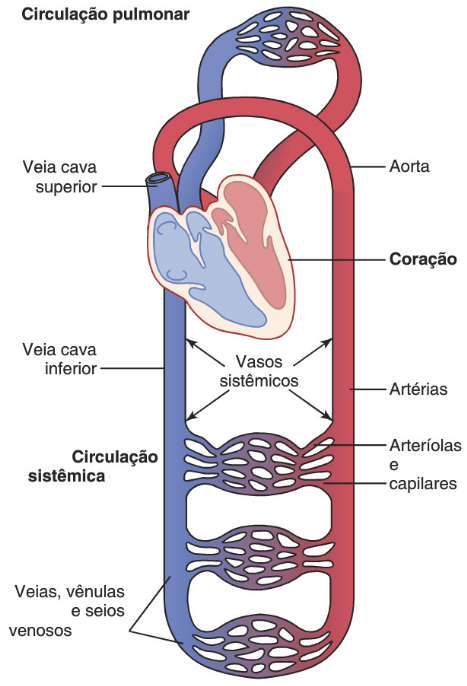
\includegraphics[scale=0.4]{figuras/revisao-sistema-circulatorio/sistema-circulatorio-humano.png}
  \fonte{Adaptado de~\cite{Hall2011}.}
  \label{fig:sistema-circulatorio}
\end{figure}

Nas ilustrações do sistema circulatório (vide Figura~\ref{fig:sistema-circulatorio}) a parte
do sangue transportada pelas artérias 
e arteríolas é representada na cor vermelha, enquanto que a parte transportada pelas veias e 
vênulas é representada na cor azul. Essa convenção vem do fato de que o sangue rico 
em oxigênio nas artérias tem uma cor vermelha mais intensa, entretanto o sangue rico em dióxido de 
carbono nas veias tem uma cor mais azulada.

O coração é basicamente uma poderosa e musculosa bomba pulsante, que mantém 
a nossa circulação ao gerar uma diferença de pressão em suas câmaras internas 
(átrio direito, ventrículo direito, átrio esquerdo e ventrículo esquerdo).

O sangue é um tecido conjuntivo formado por células (como hemácias -- glóbulos 
vermelhos -- e leucócitos -- glóbulos brancos), fragmentos de células 
(por exemplo, as plaquetas) e proteínas suspensas em uma matriz extracelular 
(o plasma, que é composto por proteínas, nutrientes, sais e hormônios).

Os vasos sanguíneos estão presentes por todo o corpo humano formando as vias de transporte nas 
quais o sangue é distribuído partindo do coração e retornando para ele. Os vasos são 
divididos em artérias, arteríolas, capilares, vênulas e veias. O sangue que é bombeado 
para fora do coração passa pelas artérias, que o transporta sob alta pressão e velocidade.
Para suportar essa alta pressão, as artérias possuem paredes vasculares mais espessas e 
rígidas do que dos demais vasos. O sangue nas artérias possui oxigênio ($O_2$) obtido durante 
a sua passagem pelos pulmões. No final da rede de artérias temos as arteríolas, que 
servem como uma espécie de ``condutos de controle'', que através de sua oclusão ou dilatação 
diminui ou aumenta (respectivamente) o fluxo sanguíneo liberado para os capilares.

Nos capilares ocorre a troca de líquidos, nutrientes, eletrólitos, hormônios e outras 
substâncias entre o sangue e o líquido intersticial. Para que essa troca possa acontecer,
as paredes dos capilares são bem finas e possuem minúsculos poros. Depois de passar 
pelos capilares, o sangue é direcionado para as vênulas que coalescem formando progressivamente
as veias. Nas veias, o sangue com o dióxido de carbono ($CO_2$) e outros restos metabólicos é 
transportado de volta para o coração. A pressão nas veias é mais baixa e suas paredes 
vasculares são mais finas e menos rígidas do que as paredes das artérias. 

Comparando a quantidade de sangue saindo do coração durante trinta minutos com a quantidade 
total de sangue no corpo humano, além de considerar o funcionamento das válvulas presentes nas veias,
o médico fisiologista William Harvey publicou em 1628 o seu livro ``\textit{De Motu Cordis et Sanguinis in Animalibus}''
com sua conclusão de que o sangue percorria um circuito circular no corpo~\cite{Whitteridge1978}.
Entretanto, Harvey não conseguiu visualizar como ocorria a passagem do sangue das partes periféricas das artérias para 
as partes periféricas das veias. Ele conjecturou que deveriam haver ``poros'' nessas regiões periféricas. Esses ``poros''
foram identificados décadas depois em 1661 por Malpighi como sendo os vasos capilares~\cite{Cliff1976}.

Atualmente sabemos que o ciclo do bombeamento do sangue começa no átrio direito (AD) do coração onde a pressão 
sanguínea é mais baixa (próxima de $0$ mmHg). Com a contração do AD o sangue é ejetado para 
o ventrículo direito (VD). Já a contração do VD ejeta o sangue para os pulmões 
(circulação pulmonar) onde o sangue receberá oxigênio e liberará dióxido de carbono. 
Dos pulmões o sangue volta para o coração entrando no átrio esquerdo (AE). Com a contração 
do AE o sangue é ejetado para o ventrículo esquerdo (VE). No VE a pressão sanguínea 
é mais alta (entre $80$ mmHg e $120$ mmHg) do que nas outras partes do coração,
sendo que com sua contração o sangue é ejetado para ser transportado para 
o resto do corpo (circulação sistêmica) através das artérias.
Depois de passar pelas arteríolas, capilares e vênulas, o sangue voltará ao coração pelas veias 
até chegar ao AD, onde o ciclo repetirá.

As artérias e veias formam estruturas que se assemelham a árvores com ramificações 
(ou bifurcações). Os trechos finais das árvores arteriais conectam-se aos trechos 
finais das árvores venosas através de vasos capilares, sendo que esses capilares 
apresentam uma estrutura que se assemelha a uma rede com diversas conexões em seus
pontos de interseção. Desse modo, temos um circuito que leva através das árvores arteriais 
o oxigênio, os nutrientes e os hormônios para os tecidos e retira através das árvores venosas 
o dióxido de carbono e os restos metabólicos.

O fluxo do sangue saindo do VE pela artéria aorta é intermitente devido ao fato do coração 
ser uma bomba pulsante. Entretanto, o fluxo do sangue chegando nos capilares é mais constante. 
Esse fenômeno foi tratado por Stephen Hales usando o efeito de Windkessel (``câmara de ar'')~\cite{Hales1733}.
Hales comparou o funcionamento do sistema composto pelas artérias e arteríolas 
com o funcionamento de um dispositivo de sua época usado no combate à incêndios. A Figura~\ref{fig:efeito-windkessel}
ilustra o conceito. Nota-se que mesmo se a água sair da bomba de modo intermitente, a água 
acumulada dentro da câmara de ar manterá algum fluxo mais constante saindo da mangueira. A artéria aorta 
possui uma complacência que permite se ajustar de modo a acumular um volume de sangue, que 
será liberado quando o coração não estiver ejetando sangue pelo VE.

\begin{figure}[!htb]
  \centering
  \captiondelim{: }
  \caption{Conceito do efeito Windkessel.} 
  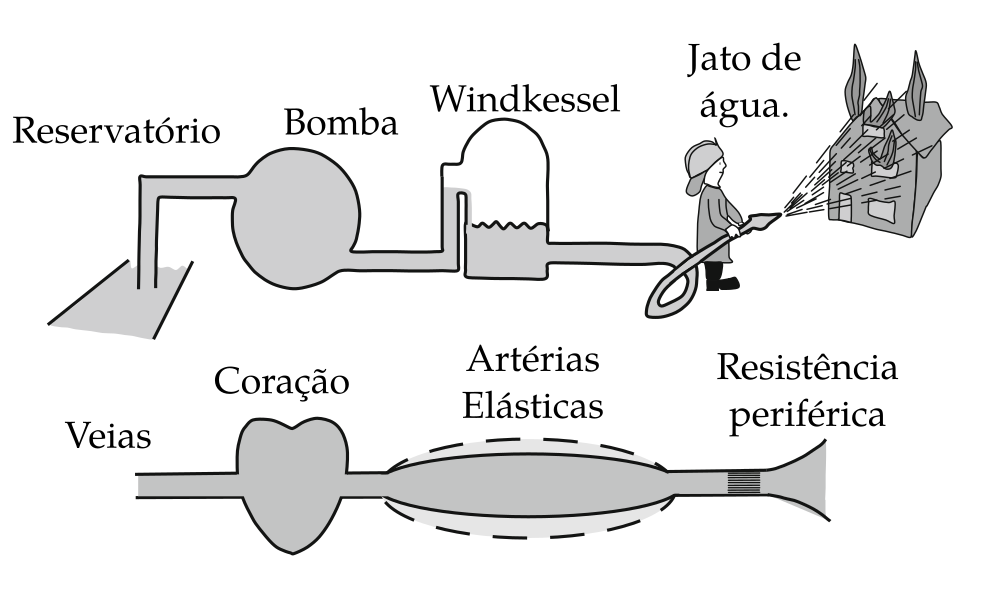
\includegraphics[scale=0.4]{figuras/revisao-sistema-circulatorio/efeito-windkessel.png}
  \fonte{Adaptado de~\cite{Westerhof2009}.}
  \label{fig:efeito-windkessel}
\end{figure}

\section{CONSTRUÇÃO DE UMA ÚNICA ÁRVORE CIRCULATÓRIA}\label{sec:cco}

Nesta seção é apresentado o método \textit{Constrained Constructive Optimization} (CCO) para 
construir uma única árvore circulatória dentro do domínio de perfusão. Este método foi inicialmente 
proposto para construir árvores vasculares 
considerando domínios bidimensionais~\cite{Schreiner1993b} e posteriormente foi
generalizado para domínios tridimensionais~\cite{Karch1999}. O método utiliza
árvores binárias adicionando sequencialmente um novo segmento com extremidade 
distal selecionada de modo aleatório no domínio de perfusão. Esse novo segmento 
é conectado a algum segmento já existente da árvore através de um ponto
de bifurcação, cuja posição é determinada de modo a minimizar uma função custo.
Durante toda a construção da árvore, condições de fluxo e pressão são levadas 
em consideração. O resultado final é uma árvore binária que possui aspectos 
morfométricos com valores próximos aos dados estatísticos de árvores vasculares 
reais encontrados na literatura especializada, 
como por exemplo o decaimento do diâmetro médio dos segmentos ao longo da árvore.
Os modelos de árvores gerados pelo método CCO utilizam às seguintes condições:

\begin{enumerate}[label=(\roman*)]
\item ramifica\c{c}\~ao binária de segmentos vasculares. Cada segmento será 
representado por um tubo rígido cilíndrico, por onde o sangue escoa em regime 
laminar e estacionário;

\item a resistência hidrodinâmica $R_i$ de um segmento $i$ é dada pela lei 
de Poiseuille~\cite{Fung1996}:
\begin{equation}
R_i = \frac{8\eta l_i}{\pi r_i^4},\label{eq:resistencia}
\end{equation}
onde $\eta$ é a viscosidade sanguínea (que será um parâmetro na simulação), 
$l_i$ e $r_i$ são, respectivamente, o comprimento e raio do segmento;

\item a queda de pressão $\Delta p_i$ ao longo do segmento $i$ é dada por:
\begin{equation}
\Delta p_i = R_i Q_i,
\label{eq:quedapressao.i}
\end{equation} 
onde $Q_i$ representa o fluxo sanguíneo através do segmento $i$;

\item a pressão $p_{term}$ na posição distal dos segmentos terminais é considerada constante;

\item $Q_{perf}$ é o fluxo sanguíneo no segmento raiz da árvore e 
$Q_{term,\,i}$ é o fluxo sanguíneo no segmento terminal $i$;

\item  a queda de pressão total $\Delta p$ da árvore é dada por 
\begin{equation}
  \Delta p = p_{perf} - p_{term},\label{eq:quedapressao}
\end{equation}
onde $p_{perf}$ é a pressão de perfusão na posi\c{c}\~ao proximal do segmento raiz;

\item em cada bifurcação, o raio do segmento pai ($r$) e dos segmentos filhos à esquerda ($r_{left}$) e 
à direita ($r_{right}$) obedecem uma lei de potência expressa por~\cite{Sherman1981}:
\begin{equation}
r^{\gamma} = r_{left}^{\gamma} + r_{right}^{\gamma},\label{eq:leibifurcacao}
\end{equation}
onde $\gamma$ é um valor pré-estabelecido no início da simulação do algoritmo CCO.

\item os segmentos são gerados de modo a minimizar a função custo (volume total da árvore)
expressa por:
\begin{equation}
  T = \pi \sum_{i=1}^{K_{tot}} l_i r_i^2,
  \label{eq:volume}
\end{equation}
onde $K_{tot}$ é o número de segmentos na árvore em cada iteração do algoritmo.
\end{enumerate}

\subsection{Critério de distância mínima}\label{sec:criterio-distancia-minima}

O Algoritmo~\ref{algo:CCOclassico} descreve a construção de uma árvore vascular pelo método CCO. 
Inicialmente o ponto proximal $\mathbf{x}_{root}$ do segmento raiz é conectado a um 
ponto $\mathbf{x}_{inew}$ escolhido de modo aleatório no domínio de perfusão $D_{perf}$.
As coordenadas desse ponto são números pseudoaleatórios seguindo uma distribuição uniforme.
Em seguida, começa um processo iterativo com $N_{term}-1$ passos. Para cada passo um novo 
ponto $\mathbf{x}_{inew}$ é gerado aleatoriamente e validado. Para validar 
esse ponto é verificado se ele está no interior do domínio de perfusão e se ele 
está a uma distância mínima $d_{min}$ de todos os segmentos criados nos passos 
anteriores (vide Figura~\ref{fig:criterio-distancia-critica}).
O valor de $d_{min}$ é diminuído a medida que o número de segmentos terminais aumenta.
Caso $\mathbf{x}_{inew}$ não passe pela validação, uma nova posição é gerada. Se esse 
ponto for gerado $N_{toss}$ vezes sem conseguir passar pela validação, então o valor de
$d_{min}$ é atualizado como $\beta d_{min}$, onde $\beta \in (0,\,1)$ é um fator
constante de redução. Para calcular a distância entre $\mathbf{x}_{inew}$ e um segmento
$\overline{AB}$, utiliza-se a distância crítica definida por
\begin{equation}
 \dist_{crit}(\mathbf{x}_{inew}, \overline{AB}) = \begin{cases}
                \dfrac{\left\|\overrightarrow{A\mathbf{x}_{inew}} \times \overrightarrow{AB}\right\|}{\left\|\overrightarrow{AB}\right\|}
                \textrm{, se }0 \leq \dfrac{\overrightarrow{A\mathbf{x}_{inew}}\cdot \overrightarrow{AB}}{\overrightarrow{AB}\cdot \overrightarrow{AB}} \leq 1;\\
                \min\{\dist(A,\,\mathbf{x}_{inew}),\, \dist(B,\,\mathbf{x}_{inew}) \}\textrm{, caso contrário;}
               \end{cases}
 \label{eq:dist-critica}
\end{equation}
onde $\dist(P,\,Q)$ representa a distância Euclidiana entre os pontos $P$ e $Q$ e 
$\min\{a,\,b\}$ representa o mínimo entre os números reais $a$ e $b$. Nota-se
que quando ocorre o caso 
$0\leq \dfrac{\overrightarrow{A\mathbf{x}_{inew}}\cdot \overrightarrow{AB}}{\overrightarrow{AB}\cdot \overrightarrow{AB}} \leq 1$ 
isso significa que pode ser traçada uma reta passando no ponto $\mathbf{x}_{inew}$
e interceptando o segmento $\overline{AB}$, de modo que essa reta seja perpendicular à $\overline{AB}$. Por isso,
nesse caso, calcula-se a distância crítica usando a
expressão $\dfrac{\left\|\overrightarrow{A\mathbf{x}_{inew}} \times \overrightarrow{AB}\right\|}{\left\|\overrightarrow{AB}\right\|}$,
que coincide com a fórmula para calcular a distância entre um ponto $\mathbf{x}_{inew}$ e a reta
passando por $A$ e $B$.

\begin{figure}[!htb]
  \centering
  \captiondelim{: }
  \caption{Ponto $\mathbf{x}_{inew}$ obedecendo à uma distância mínima $d_{min}$ em relação aos segmentos da árvore.}
  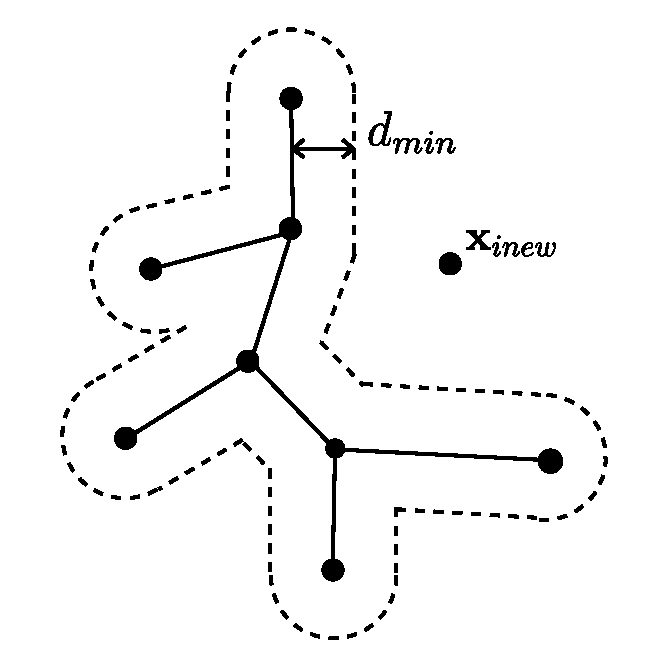
\includegraphics[scale=0.5]{figuras/modelos-computacionais-de-arvores-circulatorias/criterio-distancia-critica.pdf}
  \fonteAutor{2022}
  \label{fig:criterio-distancia-critica}
\end{figure}


\begin{algorithm}
\Dados{$D_{perf}$, $\mathbf{x}_{root}$, $Q_{perf}$, $N_{term}$, $\Delta p$, $\gamma$, $N_{con}$, $\eta$.}
  Gerar e validar uma posi\c{c}\~ao distal $\mathbf{x}_{inew}$ do segmento raiz\;
  Conectar $\mathbf{x}_{inew}$ a $\mathbf{x}_{root}$ (\textit{plantar o segmento raiz da árvore})\;
  \For{($i\gets 1$ \KwTo $N_{term}$)}{
    Gerar e validar a posi\c{c}\~ao distal $\mathbf{x}_{inew}$ de um novo segmento terminal\;
    Determinar $N \leq N_{con}$ segmentos na árvore que estão mais próximos de $\mathbf{x}_{inew}$\;
    \For{($j\gets 0$ \KwTo N)}{
      Conectar $\mathbf{x}_{inew}$ temporariamente no segmento $j$, 
      criando a bifurca\c{c}\~ao $\mathbf{x}_{ibif}$\;
      Otimizar e validar a posi\c{c}\~ao de $\mathbf{x}_{ibif}$\;
      Armazenar resultados de $\mathbf{x}_{ibif}$ na Tabela de Avaliação de Conexões (TAC)\;
      Descartar conexão temporária $\mathbf{x}_{ibif}$\;
    }
    Obter a Tabela de Avaliação de Conexões Reduzida (TAC$_r$) a partir de TAC removendo as conexões inválidas\;
    Determinar em TAC$_r$ a bifurcação ótima $\mathbf{x}_{iopt}$\;
    Conectar $\mathbf{x}_{inew}$ a $\mathbf{x}_{iopt}$ de modo permanente\;
  }
\caption{Gera\c{c}ão de árvore arterial pelo método CCO.}
\label{algo:CCOclassico}
\end{algorithm}

\subsection{Ajuste dos raios dos segmentos}\label{sec:ajuste-dos-raios}

Depois que $\mathbf{x}_{inew}$ é gerado e validado, são determinados $N \leq N_{con}$ 
segmentos da árvore que estão mais próximos dele. O valor de $N_{con}$ é fixo e fornecido 
como entrada do algoritmo. Em~\cite{Karch1999}, $N_{con} = 20$ é obtido como sendo adequado para 
encontrar a otimização local da função custo. Para cada um dos $N$ segmentos encontrados, 
uma nova árvore pode ser formada temporariamente conectando $\mathbf{x}_{inew}$ 
em um ponto do segmento encontrado. Cada bifurcação $\mathbf{x}_{ibif}$ é formada 
pelos segmentos $ibif$ (segmento de bifurcação), $icon$ (segmento de conexão)
e $inew$ (novo segmento), conforme ilustra a Figura~\ref{fig:passos-cco}. 
Inicialmente $\mathbf{x}_{ibif}$ é escolhido como o ponto médio do segmento. 
O segmento $inew$ adiciona um fluxo $Q_{inew}$ na árvore e isso 
perturba o fluxo $Q_{term,\,i}$ que os segmentos terminais devem ter. Para corrigir 
isso deve-se ajustar a resistência hidrodinâmica da árvore. Considerando que o comprimento 
dos segmentos não se altera e que as pressões de perfusão e terminal são fixas, 
efetua-se esse ajuste através da alteração dos raios dos segmentos 
criados na conexão temporária. Entretanto, ao invés de calcular diretamente 
esses raios, é efetuado o cálculo das razões entre o raio do segmento pai $ibif$ 
e seus filhos $icon$ e $inew$.

\begin{figure}[!htb]
  \centering
  \captiondelim{: }
  \caption{Ilustração dos passos básicos do Algoritmo~\ref{algo:CCOclassico}.
    (a) O ponto $\mathbf{x}_{inew}$ é escolhido aleatoriamente dentro do domínio de perfusão
    e testado para verificar o critério de distância mínima. Caso não atenda ao critério, outro
    ponto deve ser escolhido.
    (b) Conecta-se o ponto $\mathbf{x}_{inew}$ aos segmentos mais próximos na árvore. 
    Cada conexão cria um ponto $\mathbf{x}_{ibif}$.
    (c) Desloca-se a conexão $\mathbf{x}_{ibif}$ de modo a minimizar a função custo.
    }
  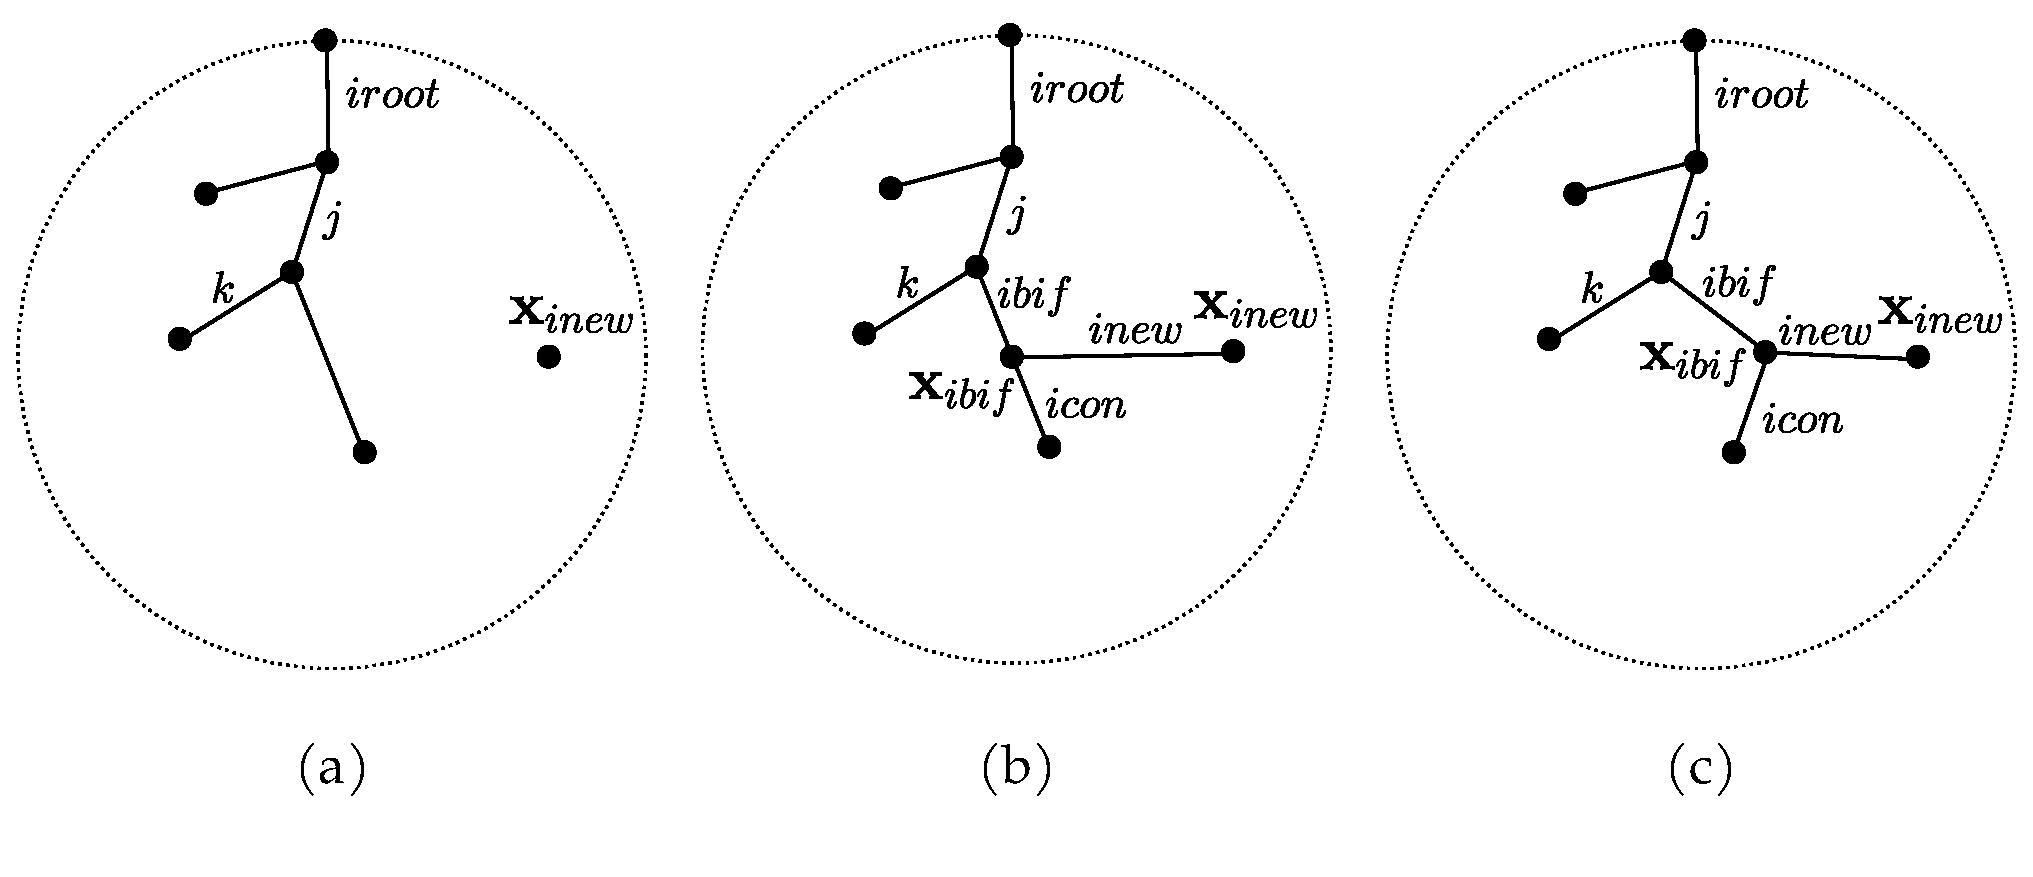
\includegraphics[scale=0.4]{figuras/modelos-computacionais-de-arvores-circulatorias/passos-algoritmo-cco.eps}
  \fonteAutor{2022}
  \label{fig:passos-cco}
\end{figure}

Como a pressão terminal é considerada constante, usando a equação~\eqref{eq:quedapressao.i} 
a razão do fluxo se dividindo no segmento $ibif$ será dada por
\begin{equation}
  R_{sub,\,icon}Q_{icon} = R_{inew}Q_{inew} \iff \frac{Q_{icon}}{Q_{inew}} = \frac{R_{inew}}{R_{sub,\,icon}}
  \iff \frac{Q_{icon}}{Q_{inew}} = \frac{\dfrac{R^*_{inew}}{r^4_{inew}}}{\dfrac{R^*_{sub,\,icon}}{r^4_{icon}}},
  \label{eq:razao.fluxo}
\end{equation}
onde $R_{sub,\,icon}$ é a resistência do segmento $icon$ incluindo suas subárvores 
esquerda e direita, $R_{inew}$ é a resistência do segmento $inew$, $R^*_{inew} = R_{inew}r^4_{inew}$
e $R^*_{sub,\,icon} = R_{sub,\,icon}r^4_{icon}$ são definidos como as resistências
reduzidas. Da equação~\eqref{eq:resistencia}, obtém-se diretamente 
$R^*_{inew} = \frac{8\eta l_{inew}}{\pi}$. Para obter $R^*_{sub,\,icon}$, devem ser 
consideradas as regras de cálculo de resistência de tubos conectados em série e em 
paralelo. Por exemplo, a resistência reduzida $R^*_{sub,\,j}$ de um segmento $j$ 
incluindo suas subárvores esquerda e direita será dada por
\begin{eqnarray}
  R^*_{sub,\,j} &=& \left[R_{j} + \left(\dfrac{1}{R_{left,\,j}} + \dfrac{1}{R_{right,\,j}}\right)^{-1}\right]r^4_j \nonumber\\ 
  &=& \frac{8\eta l_{j}}{\pi} + \left(\dfrac{r^{-4}_j}{R_{left,\,j}} + \dfrac{r^{-4}_j}{R_{right,\,j}}\right)^{-1} \nonumber\\
  &=& \frac{8\eta l_{j}}{\pi} + \left(\dfrac{r^4_{left,\,j}r^{-4}_j}{R^*_{left,\,j}} + \dfrac{r^4_{right,\,j}r^{-4}_j}{R^*_{right,\,j}}\right)^{-1} \nonumber\\
  &=& \frac{8\eta l_{j}}{\pi} + \left[\dfrac{\left(\frac{r_{left,\,j}}{r_j}\right)^4}{R^*_{left,\,j}} + \dfrac{\left(\frac{r_{right,\,j}}{r_j}\right)^4}{R^*_{right,\,j}}\right]^{-1}.
  \label{eq:resistencia.reduzida}
\end{eqnarray}

Em~\eqref{eq:resistencia.reduzida}, $R^*_{left,\,j}$ é a resistência reduzida da 
subárvore esquerda do segmento $j$ e $r_{left,\,j}$ é o raio de entrada dessa subárvore. 
De modo análogo, $R^*_{right,\,j}$ e $r_{right,\,j}$ são referentes à subárvore direita. 
Aplicando~\eqref{eq:resistencia.reduzida}, calcula-se $R^*_{sub,\,icon}$ de modo recursivo.

Isolando os raios em~\eqref{eq:razao.fluxo}, obtém-se a razão entre os raios dos 
segmentos filhos de $ibif$:
\begin{equation}
  \dfrac{r_{icon}}{r_{inew}} = \sqrt[4]{\frac{Q_{icon}R^*_{sub,\,icon}}{Q_{inew}R^*_{inew}}}.
  \label{eq:razao.raios}
\end{equation}

Por outro lado, usando~\eqref{eq:leibifurcacao} obtém-se as ``razões de bifurcação''
em relação a $ibif$:
\begin{eqnarray}
  \beta_{ibif}^{icon} &=& \dfrac{r_{icon}}{r_{ibif}} = \left[1 + \left(\dfrac{r_{icon}}{r_{inew}}\right)^{-\gamma}\right]^{-\frac{1}{\gamma}}, \label{eq:razao.bifurcacao.ibif.icon} \\ 
  & & \nonumber\\
  \beta_{ibif}^{inew} &=& \dfrac{r_{inew}}{r_{ibif}} = \left[1 + \left(\dfrac{r_{icon}}{r_{inew}}\right)^{\gamma}\right]^{-\frac{1}{\gamma}}. \label{eq:razao.bifurcacao.ibif.inew}
\end{eqnarray}

Os valores $\beta_{ibif}^{icon}$ e $\beta_{ibif}^{inew}$ são determinados 
unicamente pela razão do fluxo se dividindo em $ibif$ dada por $\frac{Q_{icon}}{Q_{inew}}$
e pela geometria da árvore através da razão $\frac{R^*_{sub,\,icon}}{R^*_{inew}}$.
Entretanto, o novo fluxo saindo por $inew$ precisa antes passar por 
$ibif$. Considerando $ibif$ e $k$ como os filhos do segmento $j$, será 
necessário então calcular as razões de bifurcação $\beta_{j}^{ibif}$ e $\beta_{j}^{k}$.
Continuando esse raciocínio, devem ser calculadas todas as razões de bifurcação dos 
segmentos no único caminho subindo a árvore a partir de $ibif$ até o segmento 
raiz ($iroot$). Nesse procedimento apenas as razões de bifurcação são armazenadas, 
não havendo necessidade de armazenar o valor dos raios dos segmentos. 
Quando for necessário o valor do raio do segmento $j$, ele pode ser obtido por
\begin{equation}
 r_j = r_{iroot} \prod_{k \in \textrm{path}(j, iroot)} \beta_{k},
 \label{eq:raio.segmento.j}
\end{equation}
onde $\beta_{k}$ é a razão de bifurcação entre o segmento $k$ e seu respectivo pai e 
$\textrm{path}(j, iroot)$ é o único caminho subindo a árvore a partir de $j$ até 
o segmento raiz ($iroot$). O valor de $r_{iroot}$ é obtido por
\begin{equation}
 r_{iroot} = \sqrt[4]{\dfrac{R^{*}_{sub,iroot}}{R_{sub,iroot}}} = \sqrt[4]{R^{*}_{sub,iroot}\dfrac{Q_{perf}}{\Delta p}},
 \label{eq:raio.iroot}
\end{equation}
onde $\Delta p = p_{perf} - p_{term}$ e $R_{sub,iroot}$ acaba denotando a resistência hidrodinâmica total da árvore.

Até aqui foram determinadas $N$ árvores temporárias, cada uma com seus valores 
para $\mathbf{x}_{ibif}$ e suas atualizações da razão das bifurcações. A posição de 
cada $\mathbf{x}_{ibif}$ será ainda otimizada de modo a minimizar a função custo 
dada por~\eqref{eq:volume}.

\subsection{Otimização geométrica}\label{sec:otimizacao-geometrica}

A nova posição de $\mathbf{x}_{ibif}$ será localizada
através de busca exaustiva dentro da região interna do triângulo 
formado pelos três pontos nos segmentos $ibif$, $inew$ e $icon$ que são distintos de $\mathbf{x}_{ibif}$.
Esse triângulo está contido no chamado plano de bifurcação~\cite{Karch1999}. 
Considera-se um mapeamento do triângulo de referência formado por $P_{i} = (0,\,0)$, 
$P_{j} = (1,\,0)$ e $P_{inew} = (0,\,1)$ com o triângulo formado pelos pontos 
$\mathbf{x}_{i}$, $\mathbf{x}_{j}$ e $\mathbf{x}_{inew}$ conforme ilustrado na 
Figura~\ref{fig:otimizacao-ponto-bifurcacao}. O mapeamento 
$\mathrm{map}:\mathbb{R}^2\to\mathbb{R}^3$ é definido tal que $\mathrm{map}(P_i) = \mathbf{x}_{i}$, 
$\mathrm{map}(P_j) = \mathbf{x}_{j}$ e $\mathrm{map}(P_{inew}) = \mathbf{x}_{inew}$. 
Esse mapeamento pode ser dado por:
\begin{equation}
  \mathrm{map}(a,\,b) = (1 - a - b)\mathbf{x}_{i} + a\mathbf{x}_{j} + b\mathbf{x}_{inew}
  \label{eq:mapeamento-bifucacao}
\end{equation}

Considere então os pontos $P_{ibif} = \left(\dfrac{m}{n},\,\dfrac{k}{n}\right)$, com $n > 1$ um 
número natural, $k = 0$, 1, 2,\ldots, $n$ e $m = 0$, 1, \ldots, $(n-k)$. A função custo~\eqref{eq:volume} 
será avaliada considerando $\mathbf{x}_{ibif} = \mathrm{map}(P_{ibif})$ e o menor valor será 
armazenado. Nas simulações realizadas neste trabalho, adotou-se $n = 5$ para tentar reduzir o 
custo computacional nesta etapa de otimização do algoritmo. Nota-se que isso significa dividir cada 
lado do triângulo de referência em cinco partes iguais.

\begin{figure}[!htb]
  \centering
  \captiondelim{: }
  \caption{Mapeamento para localizar a posição ótima de $\mathbf{x}_{ibif}$ que minimiza a função custo~\eqref{eq:volume}.}
  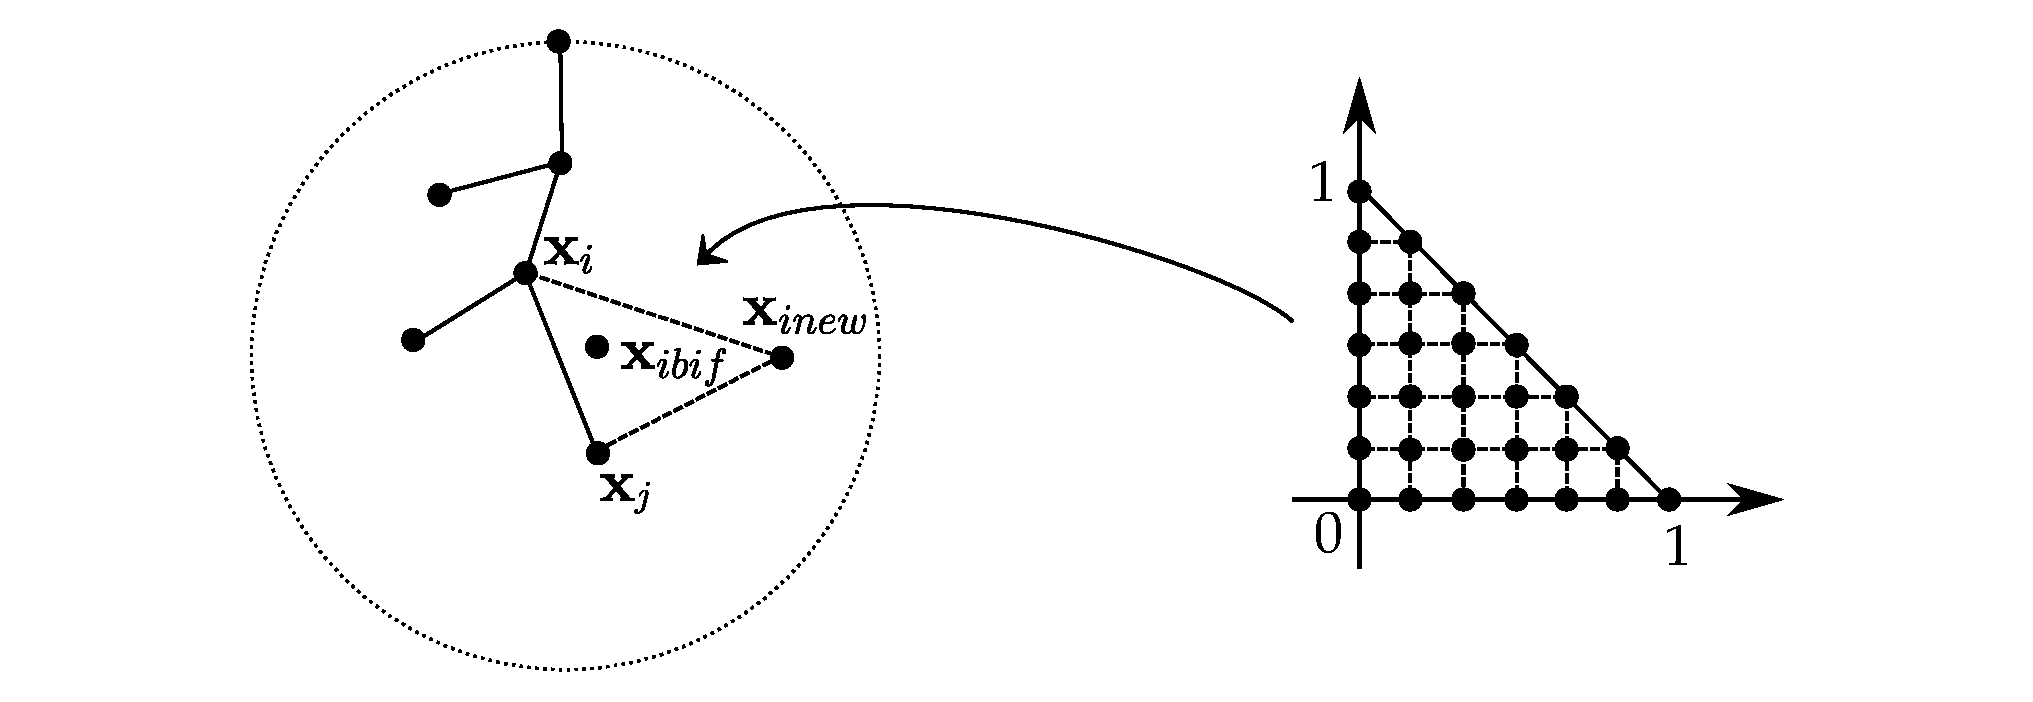
\includegraphics[width=\textwidth]{figuras/modelos-computacionais-de-arvores-circulatorias/otimizacao-do-ponto-de-bifurcacao.eps}
  \fonteAutor{2022}
  \label{fig:otimizacao-ponto-bifurcacao}
\end{figure}

A posição encontrada será válida se $\mathbf{x}_{ibif}$ permanecer no domínio de perfusão e 
os comprimentos dos segmentos $ibif$, $inew$ e $icon$ forem maiores do que seus respectivos 
diâmetros.

\subsection{Otimização estrutural}\label{sec:otimizacao-estrutural}

Como a posição de $\mathbf{x}_{ibif}$
será alterada, isso implica em alterar o comprimento de $ibif$, $inew$ e $icon$ e consequentemente
a resistência hidrodinâmica da árvore. Desse modo, devem ser atualizadas as razões de bifurcação 
desde esses segmentos até a raiz da árvore. Os resultados de cada árvore temporária serão armazenados 
na Tabela de Avaliação de Conexão (TAC). A TAC será posteriormente reduzida para TAC$_r$, na qual as 
conexões inválidas serão removidas (isto é, remover os casos onde o $inew$ intercepte algum segmento 
existente na árvore). Caso TAC$_r$ seja vazia, um novo ponto $\mathbf{x}_{inew}$ deve ser 
escolhido e as iterações são reiniciadas. Caso contrário, em TAC$_r$ é determinada a bifurcação 
ótima $\mathbf{x}_{iopt}$, ou seja, que gera o menor valor para a função custo. A bifurcação 
$\mathbf{x}_{iopt}$ é conectada a $\mathbf{x}_{inew}$ de modo permanente. Desse modo, a árvore 
passa a ter um segmento terminal a mais e o algoritmo vai reiniciar suas iterações até que seja 
atingido a quantidade $N_{term}$ de terminais.

\subsection{Interseção entre segmentos}\label{sec:intersecao-entre-segmentos}

Durante o processo de otimização geométrica (conforme descrito na Seção~\ref{sec:otimizacao-geometrica}) são 
alterados os segmentos $s_c$ e seus filhos $s_{i-1}$ e $s_{i}$ (onde $s_{i-1}$ é o segmento de conexão referente 
ao segmento terminal $s_i$). Eventualmente essa alteração pode fazer com que $s_c$, $s_{i-1}$ ou $s_i$ 
intercepte algum outro segmento da árvore. Caso ocorra alguma interseção, isso deve ser identificado 
durante a redução da Tabela de Avaliação de Conexões (conforme descrito na Seção~\ref{sec:otimizacao-estrutural}).
Para determinar se existe interseção entre o segmento $s_u$ (com $u=c$, $u=i-1$ ou $u=i$) e um outro segmento 
$s_v$ da árvore, considera-se dois casos distintos conforme esteja-se trabalhando com pontos em $\mathbb{R}^2$ ou 
com pontos em $\mathbb{R}^3$.

\subsubsection{Segmentos no $\mathbb{R}^2$}\label{subsec:intersecao-2d}

Suponha que os pontos proximal e distal do segmento $s_u$ sejam, respectivamente, 
$A = (x_A,\, y_A)$ e $B = (x_B,\, y_B)$. 
Por outro lado, suponha que os pontos proximal e distal do segmento $s_v$ sejam, respectivamente, 
$C = (x_C,\, y_C)$ e $D = (x_D,\, y_D)$. 
As retas suporte $u$ e $v$, respectivamente, de $s_u$ e $s_v$ são dadas por:
\begin{eqnarray}
  u: & X = A + \lambda_u\overrightarrow{AB}\label{eq:reta-suporte-do-segmento-su}, \\
  v: & X = C + \lambda_v\overrightarrow{CD}\label{eq:reta-supor	te-do-segmento-sv}.
\end{eqnarray}

Nota-se que os pontos de $s_u$ e $s_v$ são tais que, respectivamente, 
tem-se $\lambda_u\in[0, 1]$ e $\lambda_v\in[0, 1]$. Além disso, a interseção entre 
as retas $u$ e $v$ ocorre quando:
\begin{equation}
  A + \lambda_u\overrightarrow{AB} = C + \lambda_v\overrightarrow{CD}.
  \label{eq:intersecao-segmentos-caso-2d}
\end{equation}

A solução dessa equação será dada por:
\begin{equation}
  \begin{cases}
    \lambda_u = \dfrac{(x_D - x_C)(y_C - y_A) - (x_C - x_A)(y_D - y_C)}{(x_D - x_C)(y_B - y_A) - (x_B - x_A)(y_D - y_C)}\\ \\
    \lambda_v = \dfrac{(x_B - x_A)(y_C - y_A) - (x_C - x_A)(y_B - y_A)}{(x_D - x_C)(y_B - y_A) - (x_B - x_A)(y_D - y_C)}
  \end{cases}
  \label{eq:solucao-sistema-intersecao-segmentos-caso-2d}
\end{equation}

Quando as retas $u$ e $v$ são paralelas não há interseção e portanto esse sistema não tem solução.
Considera-se que esse seja o caso quando
\begin{equation}
  |(x_D - x_C)(y_B - y_A) - (x_B - x_A)(y_D - y_C)| < \varepsilon,
  \label{eq:solucao-tolerancia-sistema-intersecao-segmentos-caso-2d}
\end{equation}
onde $\varepsilon = 10^{-12}$ é uma tolerância.

Por outro lado, quando $u$ e $v$ não são paralelas, elas se interceptam e o sistema tem solução.
Considera-se que a interseção ocorre sobre $s_u$ e $s_v$ quando: 
\begin{equation}
  \begin{cases}
    0 < \lambda_u < 1 + \dfrac{r_u + r_v}{\left\|\overrightarrow{AB}\right\|} \\
    \\
    0 < \lambda_v < 1 + \dfrac{r_u + r_v}{\left\|\overrightarrow{CD}\right\|}
  \end{cases},
  \label{eq:solucao-tolerancia-intersecao-segmentos-caso-2d}
\end{equation}
onde $r_u$ e $r_v$ são, respectivamente, os raios de $s_u$ e $s_v$.

\subsubsection{Segmentos no $\mathbb{R}^3$}\label{subsec:intersecao-3d}

Suponha que os pontos proximal e distal do segmento $s_u$ sejam, respectivamente, 
$A = (x_A,\, y_A,\, z_A)$ e $B = (x_B,\, y_B,\, z_B)$. 
Por outro lado, suponha que os pontos proximal e distal do segmento $s_v$ sejam, respectivamente, 
$C = (x_C,\, y_C,\, z_C)$ e $D = (x_D,\, y_D,\, z_D)$. Além disso, 
sejam $P = (x_P, y_P, z_P)$ um ponto sobre $s_u$ e 
$Q = (x_Q, y_Q, z_Q)$ um ponto sobre $s_v$. As retas suporte $u$ e $v$, 
respectivamente, de $s_u$ e $s_v$ são dadas por:
\begin{eqnarray}
  u: & X = A + \lambda_u\overrightarrow{AB}\label{eq:reta-suporte-do-segmento-su-3d}, \\
  v: & X = C + \lambda_v\overrightarrow{CD}\label{eq:reta-suporte-do-segmento-sv-3d}.
\end{eqnarray}

Se o vetor $\overrightarrow{PQ}$ for ortogonal ao mesmo tempo à $s_u$ e $s_v$, então seu módulo
será o menor possível. Nesse caso, tem-se o sistema de equações:
\begin{equation}
  \begin{cases}
    P = A + \lambda_u\overrightarrow{AB}\\
    Q = C + \lambda_v\overrightarrow{CD}\\
    \langle \overrightarrow{PQ}, \, \overrightarrow{AB}\rangle = 0\\
    \langle \overrightarrow{PQ}, \, \overrightarrow{CD}\rangle = 0\\
  \end{cases}
  \label{eq:intersecao-segmentos-caso-3d}
\end{equation}
 
Nota-se que $P$ e $Q$ são tais que, respectivamente, 
tem-se $\lambda_u\in[0, 1]$ e $\lambda_v\in[0, 1]$. Reescrevendo~\eqref{eq:intersecao-segmentos-caso-3d} de forma mais
conveniente, obtém-se que:
\begin{equation}
  % <AB, AB>*r - <AB, CD>*s = <AC, AB>
  % <AB, CD>*r - <CD, CD>*s = <AC, CD>
  \begin{cases}
    \langle \overrightarrow{AB}, \, \overrightarrow{AB}\rangle \lambda_u - \langle \overrightarrow{AB}, \, \overrightarrow{CD}\rangle\lambda_v = \langle \overrightarrow{AC}, \, \overrightarrow{AB}\rangle \\
    \langle \overrightarrow{AB}, \, \overrightarrow{CD}\rangle \lambda_u - \langle \overrightarrow{CD}, \, \overrightarrow{CD}\rangle\lambda_v = \langle \overrightarrow{AC}, \, \overrightarrow{CD}\rangle
  \end{cases}.
  \label{eq:sistema-intersecao-segmentos-caso-3d}
\end{equation}

A solução desse sistema será dada por:
\begin{equation}
  \begin{cases}
    \lambda_u = \dfrac{\langle \overrightarrow{AB}, \, \overrightarrow{CD}\rangle \langle \overrightarrow{AC}, \, \overrightarrow{CD}\rangle - \langle \overrightarrow{AC}, \, \overrightarrow{AC}\rangle \langle \overrightarrow{CD}, \, \overrightarrow{CD}\rangle}{\langle \overrightarrow{AB}, \, \overrightarrow{CD}\rangle ^2 - \langle \overrightarrow{AB}, \, \overrightarrow{AB}\rangle \langle \overrightarrow{CD}, \, \overrightarrow{CD}\rangle}\\ \\
    \lambda_v = \dfrac{\langle \overrightarrow{AB}, \, \overrightarrow{AB}\rangle \langle \overrightarrow{AC}, \, \overrightarrow{CD}\rangle - \langle \overrightarrow{AC}, \, \overrightarrow{AB}\rangle \langle \overrightarrow{AB}, \, \overrightarrow{CD}\rangle}{\langle \overrightarrow{AB}, \, \overrightarrow{CD}\rangle ^2 - \langle \overrightarrow{AB}, \, \overrightarrow{AB}\rangle \langle \overrightarrow{CD}, \, \overrightarrow{CD}\rangle}
  \end{cases}
  \label{eq:solucao-sistema-intersecao-segmentos-caso-3d}
\end{equation}

Quando as retas $u$ e $v$ são paralelas existem infinitos vetores $\overrightarrow{PQ}$ 
que atendem ao sistema~\eqref{eq:sistema-intersecao-segmentos-caso-3d} e portanto ele
possui infinitas soluções. Considera-se que esse seja o caso quando
\begin{equation}
  \left|\langle \overrightarrow{AB}, \, \overrightarrow{CD}\rangle ^2 - \langle \overrightarrow{AB}, \, \overrightarrow{AB}\rangle \langle \overrightarrow{CD}, \, \overrightarrow{CD}\rangle\right| < \varepsilon,
  \label{eq:solucao-tolerancia-sistema-intersecao-segmentos-caso-3d}
\end{equation}
onde $\varepsilon = 10^{-6}$ é uma tolerância.

Por outro lado, quando $u$ e $v$ não são paralelas existe um único vetor $\overrightarrow{PQ}$ 
que atende ao sistema~\eqref{eq:sistema-intersecao-segmentos-caso-3d} e portanto ele
possui uma única solução. Considera-se que haverá interseção sobre $s_u$ e $s_v$ quando: 
\begin{equation}
  \begin{cases}
    0 < \lambda_u < 1 \\
    0 < \lambda_v < 1 \\
	\left\|\overrightarrow{PQ}\right\| < r_u + r_v
  \end{cases},
  \label{eq:solucao-tolerancia-intersecao-segmentos-caso-3d}
\end{equation}
onde $r_u$ e $r_v$ são, respectivamente, os raios de $s_u$ e $s_v$.

\section{CONSTRUÇÃO DE MÚLTIPLAS ÁRVORES ARTERIAIS}\label{sec:construcao-de-multiplas-arvores}

O método CCO~\cite{Karch1999,Schreiner1993b} cria apenas uma árvore vascular por vez.
Entretanto, em geral encontra-se mais de uma árvore presente nos tecidos e órgãos. 
A partir de artérias fonte surgem as artérias perfurantes, sendo que a partir dessas,
continuando a vascularização, podemos ter outras árvores vasculares dentro de um 
mesmo domínio de perfusão. Essas árvores podem competir entre si na distribuição do fluxo sanguíneo.
Além disso, podemos encontrar árvores de tipos diferentes (por exemplo, 
uma arterial e outra venosa).

Para a construção de múltiplas árvores em um mesmo domínio de perfusão 
podemos adotar duas estratégias básicas. Uma primeira estratégia pode ser 
subdividir o domínio de perfusão em subdomínios e aplicar o método CCO 
em cada um deles para construir sua respectiva árvore.
Em~\cite{Blanco2013}, um método variacional é utilizado para efetuar essa subdivisão
do domínio.

Por outro lado, uma segunda estratégia envolve alterar o próprio método
CCO de modo a criar mais de uma árvore simultaneamente sem subdividir o domínio de
perfusão. Em~\cite{Queiroz2018}, o método CCO foi adaptado para construir
duas ou mais árvores de modo a ter seus segmentos terminais conectados em 
seus pontos distais. Essa conexão representa a escala da microcirculação, na qual encontramos a 
rede de vasos capilares. As árvores criadas não competem entre si pelo fluxo
sanguíneo durante a construção da floresta. 
Já em~\cite{Jaquet2019} o método CCO foi alterado para construir as árvores 
de modo a alcançar um determinado percentual do fluxo sanguíneo total, sendo que as árvores
competem pelo fluxo durante a construção. Diferente da proposta em~\cite{Queiroz2018}, 
essas árvores não apresentam uma conexão nos pontos distais de seus segmentos terminais.

\subsection{Construção de árvores arteriais e venosas acopladas}\label{subsec:arvores-arterial-venosa}

Suponha que o modelo geométrico de um sistema vascular arteriovenoso seja formado por 
duas ou mais árvores circulatórias conectadas em seus segmentos vasculares terminais. Para a construção 
deste modelo, utilizou-se o Algoritmo~\ref{algo:CCOVenosoArterial} baseado no método CCO~\cite{Queiroz2018}.
As árvores deste modelo atendem as mesmas condições do CCO descritas na Seção~\ref{sec:cco}. A 
Figura~\ref{fig:CCOVenosoArterial} ilustra os passos do Algoritmo~\ref{algo:CCOVenosoArterial} 
para construir um modelo com duas árvores vasculares ($N_{trees} = 2$), cada uma com 
dois segmentos terminais ($N_{term} = 2$).

\begin{figure}[!htb]
  \centering
  \captiondelim{: }
  \caption{Representa\c{c}\~ao da gera\c{c}\~ao de um sistema vascular arteriovenoso. 
  A cor azul representa a árvore venosa e a vermelha a árvore arterial.
  (a) Conexão de $\mathbf{x}_{inew}$ com $\mathbf{x}_{prox}^1$ e $\mathbf{x}_{prox}^2$.
  (b) Conexão de $\mathbf{x}_{inew}$ com $\mathbf{x}_{ibif}^1$ e $\mathbf{x}_{ibif}^2$.
  (c) Deslocamento de $\mathbf{x}_{ibif}^1$ e $\mathbf{x}_{ibif}^2$ de modo a otimizar a função custo.}
  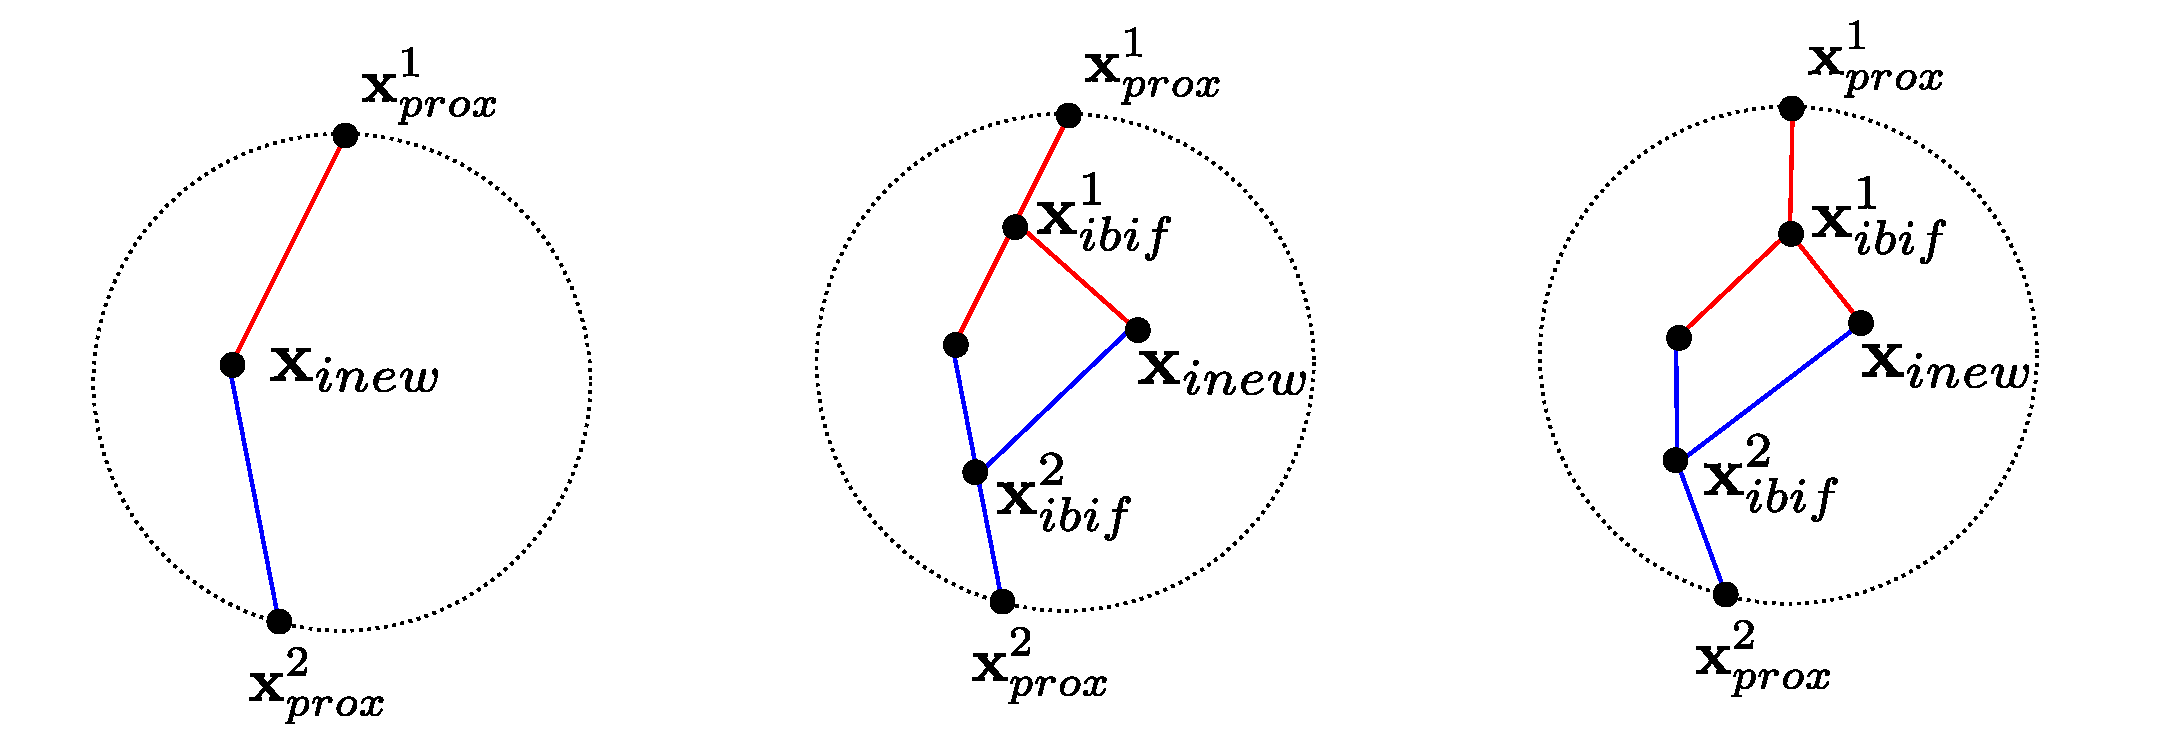
\includegraphics[width = \textwidth]{figuras/modelos-computacionais-de-arvores-circulatorias/passos-algoritmo-arteriovenoso.eps}

  (a) \hspace{0.33\textwidth} (b) \hspace{0.33\textwidth} (c)
  \fonteAutor{2022}
  \label{fig:CCOVenosoArterial}
\end{figure}

\begin{algorithm}
\Dados{$D_{perf}$, $\mathbf{x}_{prox}^t$, $Q_{perf}^t$, $N_{term}$, $\Delta p^t$, $\gamma$, $N_{trees}$.}
  Fixar as posi\c{c}\~oes proximais dos segmentos raízes $\mathbf{x}_{prox}^t$ no domínio de perfusão\; 
  Gerar e validar a posi\c{c}\~ao terminal $\mathbf{x}_{inew}$ dos segmentos raízes\;
  \For{$t \gets 1$ \textbf{até} $N_{trees}$}{
    Conectar $\mathbf{x}_{inew}$ a $\mathbf{x}_{prox}^t$ (\textit{coloca segmento raiz da árvore $t$})\;
  }
  $k_{term} = 1$\;
  \While{($k_{term} < N_{term}$)}{    
    Gerar e validar a posi\c{c}\~ao distal $\mathbf{x}_{inew}$ de um novo segmento terminal\;
    Conectar $\mathbf{x}_{inew}$ a um segmento de cada árvore $t$ criando novas bifurca\c{c}\~oes $\mathbf{x}_{ibif}^t$\;
    Otimizar a posi\c{c}\~ao de $\mathbf{x}_{ibif}^t$\;
    $k_{term} = k_{term} + 1$\;
  }
  \caption{Gera\c{c}ão de sistema vascular arteriovenoso com $N_{trees}$ árvores~\cite{Queiroz2013,Queiroz2018}.}
  \label{algo:CCOVenosoArterial}
\end{algorithm}

O Algoritmo~\ref{algo:CCOVenosoArterial} funciona basicamente como o Algoritmo~\ref{algo:CCOclassico} 
do método CCO, mas vale destacar os seguintes pontos:
\begin{itemize}
 \item para cada árvore $t$ ($t=1,\ldots,N_{trees}$), a posi\c{c}\~ao proximal do segmento raiz ($\mathbf{x}_{prox}^t$), 
 o fluxo no segmento raiz ($Q_{perf}^t$) e a queda de pressão total ($\Delta p^t$) são dados de entrada do algoritmo.
 O valor de $N_{trees}$ pode ser arbitrário, em particular $N_{trees}$ = 2 no caso do sistema vascular 
 renal;
 
 \item tanto na linha 2 como na linha 8 do Algoritmo~\ref{algo:CCOVenosoArterial}, a posi\c{c}\~ao $\mathbf{x}_{inew}$
 gerada (aleatoriamente) só é validada se atender um critério de 
 distância~\cite{Queiroz2013, Schreiner1993b} em rela\c{c}\~ao aos segmentos já existentes 
 de cada árvore $t$ (caso contrário outra posição é gerada);

 \item cada nova posi\c{c}\~ao $\mathbf{x}_{inew}$ será conectada em mais de uma árvore a cada passo; 
  
 \item ao conectar a posi\c{c}\~ao $\mathbf{x}_{inew}$ em segmentos das árvores $t$, criamos novas bifurcações 
 ($\mathbf{x}_{ibif}^t$) que necessitam ser otimizadas em cada árvore de modo a minimizar a sua respectiva 
 função custo~\eqref{eq:volume}.
\end{itemize}

\subsection{Construção de florestas de árvores arteriais}\label{subsec:floresta-vascular}

Em~\cite{Jaquet2019}, é proposto um algoritmo baseado no método CCO, 
resumido conforme o fluxograma ilustrado na Figura~\ref{algo:CCOFlorestaDeArvores}, 
que realiza a construção de uma floresta de árvores vasculares. 
Suponha que serão criadas $N_{trees}$ árvores em um volume de perfusão $D_{perf}$, 
cada uma com um fluxo alvo $q_{targ}^t$, onde $t = 1,\,2,\,\ldots,\,N_{trees}$. 

Inicialmente, os pontos $\mathbf{x}_{inew}^t$ são gerados aleatoriamente. 
Cada ponto $\mathbf{x}_{inew}^t$ é 
considerado válido se estiver dentro do domínio de perfusão e se sua distância ao 
ponto $\mathbf{x}_{root}^t$ (ponto proximal do segmento raiz da árvore $t$) for 
menor ou igual a $l_{max}^t$ dado por:
\begin{equation}
 l_{max}^t = d_{cn}^t \dfrac{q_{targ}^t}{q_{targ}^{cn} + q_{targ}^t},
 \label{eq:criterio.distancia.raiz}
\end{equation}
onde $d_{cn}^t$ é a distância entre o ponto $\mathbf{x}_{root}^t$ 
e o ponto $\mathbf{x}_{root}^i$ (com $i\neq t$) mais próximo 
e $q_{targ}^{cn}$ é o fluxo alvo da árvore $i$. Após esta etapa de geração e validação, 
o ponto $\mathbf{x}_{inew}^t$ será conectado ao ponto $\mathbf{x}_{root}^t$ formando
o segmento raiz da árvore $t$.

Durante o crescimento da floresta é criado uma competição entre as 
árvores para ocupar o domínio de perfusão. Para isso, é analisado o fluxo relativo entre elas.
Supondo que a árvore $b$ tenha o maior fluxo
alvo $q_{targ}^b$, o fluxo relativo da árvore $t\neq b$ no passo $K_{term}$ da
iteração é dado por:
\begin{equation}
 \chi_{K_{term}}^t = \dfrac{q_{K_{term}}^t}{q_{K_{term}}^b}\textrm{.}
 \label{eq:fluxo.relativo.temporario}
\end{equation}

Esse fluxo relativo é comparado com o fluxo alvo relativo:
\begin{equation}
 \chi_{targ}^t = \dfrac{q_{targ}^t}{q_{targ}^b}
 \label{eq:fluxo.relativo.total}
\end{equation}

Define-se que a árvore $t$ está ativa se $\chi_{targ}^t > \chi_{K_{term}}^t$ e como
inativa caso contrário. Em relação a árvore $b$, marca-se como ativa se
$q_{targ}^b > q_{K_{term}}^b$ e como inativa caso contrário. A cada passo do processo de
crescimento da floresta, um novo segmento terminal é adicionado a uma das árvores ativas 
de modo que o volume total da floresta (isto é, a soma dos volumes de cada árvore calculado 
conforme~\eqref{eq:volume}) seja mínimo.

\begin{figure}
  \centering
  \caption{Fluxograma do algoritmo de gera\c{c}ão de floresta de árvores vasculares conforme~\cite{Jaquet2019}.}
  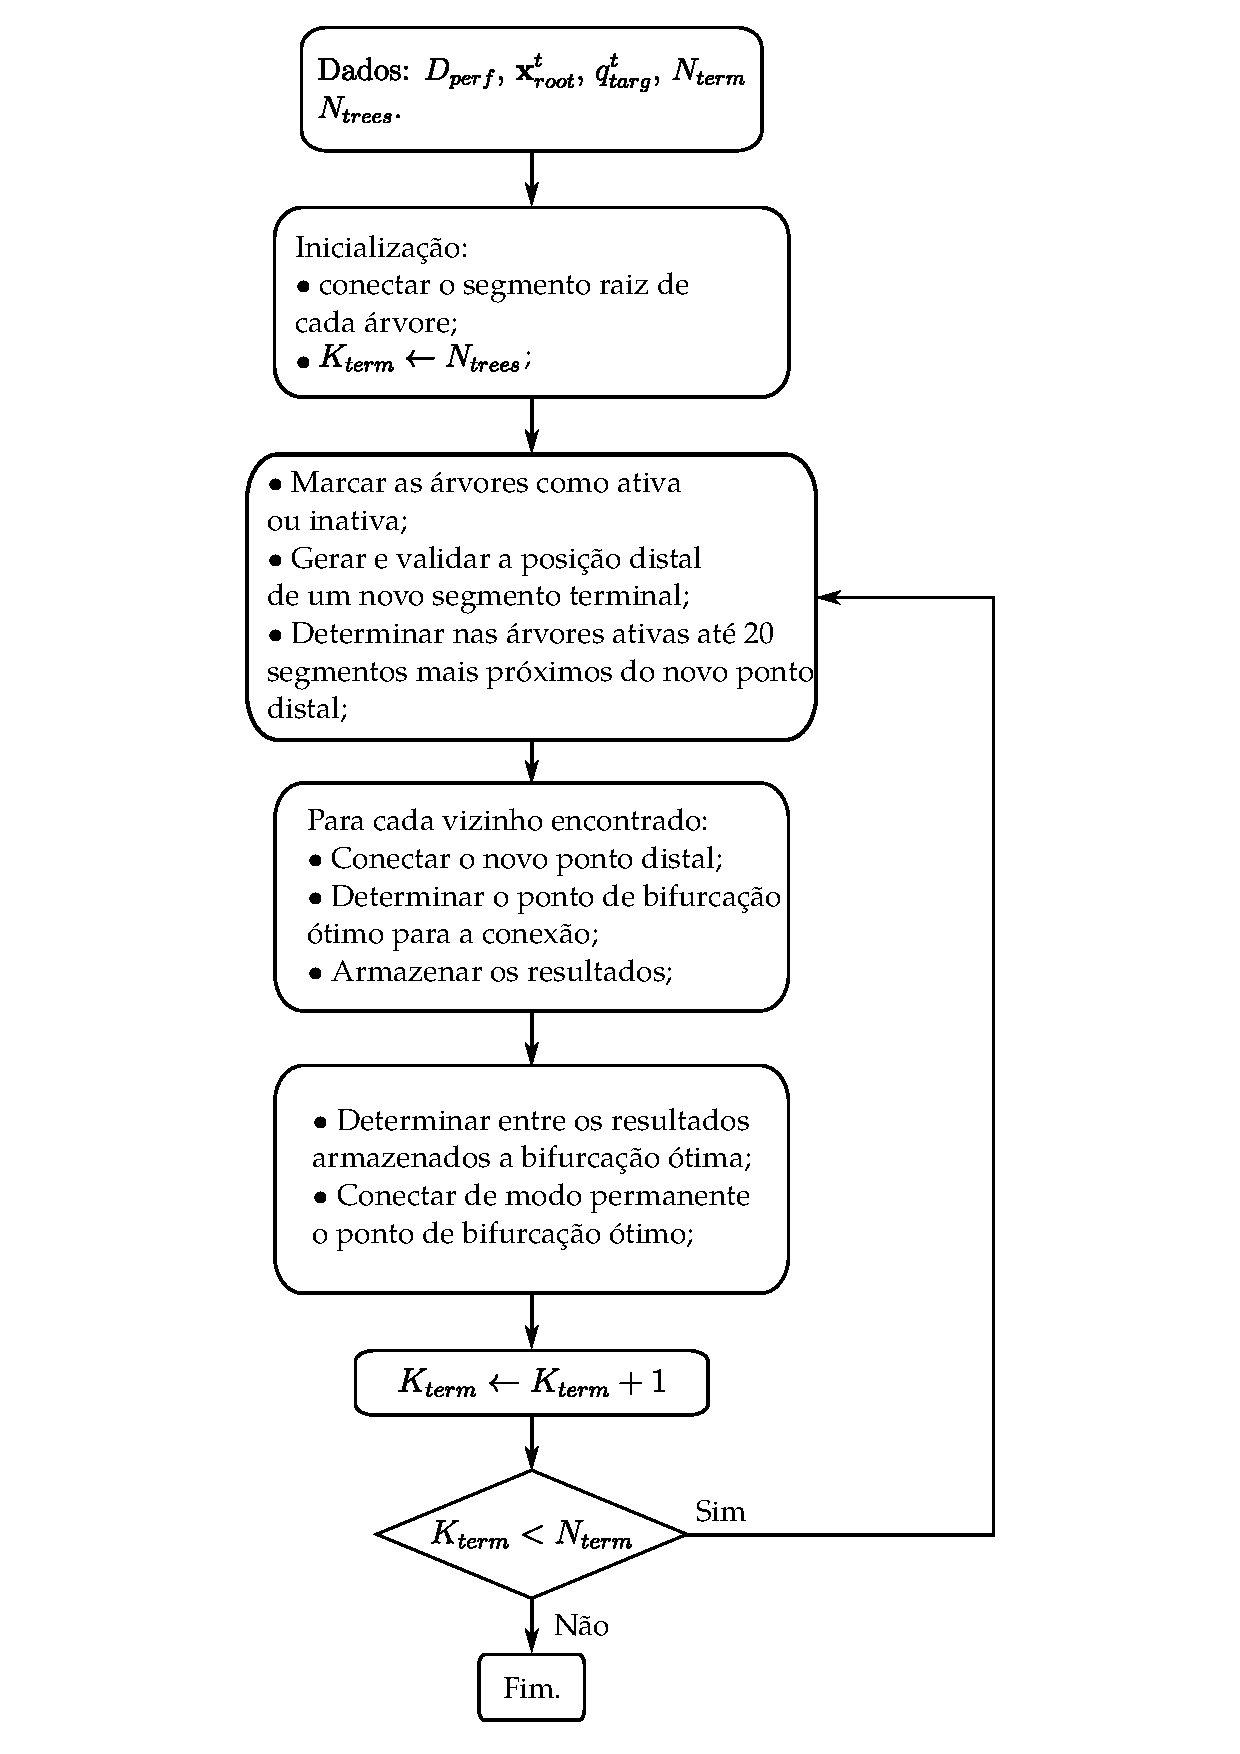
\includegraphics[scale=0.75]{figuras/modelos-computacionais-de-arvores-circulatorias/fluxograma-algoritmo-jaquet.pdf}
  \fonteAutor{2022}
  \label{algo:CCOFlorestaDeArvores}
\end{figure}

Para o ponto $\mathbf{x}_{inew}$ ser válido o segmento mais próximo dele deve estar em uma 
árvore ativa. Considerando as árvores ativas para as quais $\mathbf{x}_{inew}$ for válido, 
são encontrados os $N \leq 20$ segmentos mais próximos deste ponto (isto é, aqui considera-se 
$N_{con} = 20$ conforme~\cite{Karch1999}). Para cada segmento encontrado, 
uma conexão temporária é determinada e otimizada 
seguindo ideias semelhantes ao método CCO explicadas na Seção~\ref{sec:cco}
(a otimização geométrica da conexão é feita como em~\cite{Kamiya1972}).

Para determinar os subdomínios ocupados em cada simulação, foi 
construído um Diagrama de Voronoi~\cite{Aurenhammer2004}. Dados os pontos distais dos terminais das 
árvores, $P_1$, $P_2$, \ldots, $P_n$ (com $n = N_{term}$),
o domínio de perfusão $D_{perf}$ é dividido em 
$n$ subregiões $D_1$, $D_2$, \ldots, $D_n$ tais que:
\begin{equation}
 D_i = \{P\in D_{perf} \,|\, \dist(P,P_i) < \dist(P, P_j),\, \forall j\neq i\}\textrm{.}
 \label{def:diagrama-voronoi}
\end{equation}

O território ocupado por uma árvore $t$ será composto pela união das subregiões 
$D_i$ tais que $P_i$ seja um ponto pertencente à árvore $t$. Em~\cite{Jaquet2019}, 
é exibido que o território ocupado por uma árvore $t$ segue um percentual (em relação 
ao território total do domínio de perfusão $D_{perf}$) que é compatível com o percentual 
dos fluxos alvo (em relação ao fluxo total na floresta).

Apesar do algoritmo proposto em~\cite{Jaquet2019} implementar uma estratégia de competição 
pelo fluxo de sangue entre as árvores na floresta (através da comparação 
entre $\chi_{K_{term}}^t$ e $\chi_{targ}^t$), não há no algoritmo um parâmetro 
que permita controlar a invasão de uma árvore no território da outra. 
Na Seção~\ref{sec:floresta-com-invasao} é discutida uma estratégia para
implementar esse controle.